\documentclass[tikz,border=8pt]{standalone}
% Shared look for every TikZ diagram. Load with % Shared look for every TikZ diagram. Load with % Shared look for every TikZ diagram. Load with \input{../../tools/tikz-style.tex}
\usepackage[T1]{fontenc}
\usepackage{lmodern}
\renewcommand{\sfdefault}{lmr}  % diagrams use the same serif as the text
\usetikzlibrary{arrows.meta, positioning, shapes.geometric, calc, fit, backgrounds}
\definecolor{cblue}{HTML}{4C78A8}
\definecolor{corange}{HTML}{F58518}
\definecolor{cgreen}{HTML}{54A24B}
\definecolor{cred}{HTML}{E45756}
\definecolor{cpurple}{HTML}{B279A2}
\definecolor{cgrey}{HTML}{6B6B6B}
\tikzset{
  every picture/.style={font=\sffamily, line width=1.2pt},
  box/.style={draw=#1, fill=#1!12, rounded corners=4pt, align=center, inner sep=7pt, minimum height=1.1cm},
  box/.default=cgrey,
  arrow/.style={-{Stealth[length=3mm]}, draw=cgrey, line width=1.4pt},
  title/.style={font=\sffamily\bfseries\Large},
  note/.style={font=\sffamily\small, text=cgrey, align=center},
}
\AtBeginDocument{\hyphenpenalty=10000 \exhyphenpenalty=10000}

\usepackage[T1]{fontenc}
\usepackage{lmodern}
\renewcommand{\sfdefault}{lmr}  % diagrams use the same serif as the text
\usetikzlibrary{arrows.meta, positioning, shapes.geometric, calc, fit, backgrounds}
\definecolor{cblue}{HTML}{4C78A8}
\definecolor{corange}{HTML}{F58518}
\definecolor{cgreen}{HTML}{54A24B}
\definecolor{cred}{HTML}{E45756}
\definecolor{cpurple}{HTML}{B279A2}
\definecolor{cgrey}{HTML}{6B6B6B}
\tikzset{
  every picture/.style={font=\sffamily, line width=1.2pt},
  box/.style={draw=#1, fill=#1!12, rounded corners=4pt, align=center, inner sep=7pt, minimum height=1.1cm},
  box/.default=cgrey,
  arrow/.style={-{Stealth[length=3mm]}, draw=cgrey, line width=1.4pt},
  title/.style={font=\sffamily\bfseries\Large},
  note/.style={font=\sffamily\small, text=cgrey, align=center},
}
\AtBeginDocument{\hyphenpenalty=10000 \exhyphenpenalty=10000}

\usepackage[T1]{fontenc}
\usepackage{lmodern}
\renewcommand{\sfdefault}{lmr}  % diagrams use the same serif as the text
\usetikzlibrary{arrows.meta, positioning, shapes.geometric, calc, fit, backgrounds}
\definecolor{cblue}{HTML}{4C78A8}
\definecolor{corange}{HTML}{F58518}
\definecolor{cgreen}{HTML}{54A24B}
\definecolor{cred}{HTML}{E45756}
\definecolor{cpurple}{HTML}{B279A2}
\definecolor{cgrey}{HTML}{6B6B6B}
\tikzset{
  every picture/.style={font=\sffamily, line width=1.2pt},
  box/.style={draw=#1, fill=#1!12, rounded corners=4pt, align=center, inner sep=7pt, minimum height=1.1cm},
  box/.default=cgrey,
  arrow/.style={-{Stealth[length=3mm]}, draw=cgrey, line width=1.4pt},
  title/.style={font=\sffamily\bfseries\Large},
  note/.style={font=\sffamily\small, text=cgrey, align=center},
}
\AtBeginDocument{\hyphenpenalty=10000 \exhyphenpenalty=10000}

\begin{document}
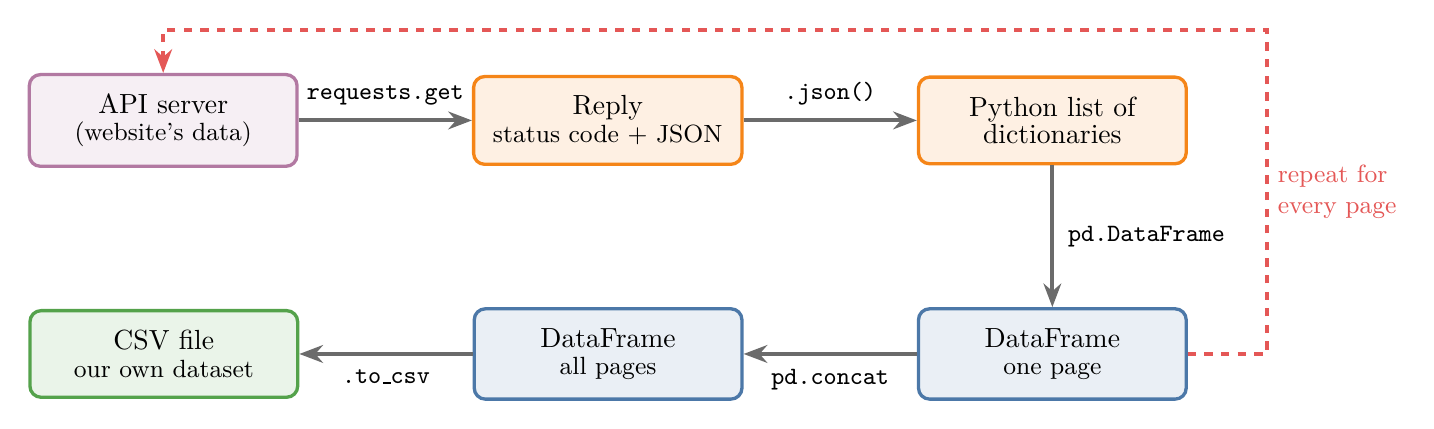
\begin{tikzpicture}[node distance=1.0cm and 2.2cm, lbl/.style={font=\ttfamily\small, fill=white, inner sep=2pt}]
  \node[box=cpurple, minimum width=3.4cm] (api) {API server\\[-2pt]\small(website's data)};
  \node[box=corange, minimum width=3.4cm, right=of api] (reply) {Reply\\[-2pt]\small status code + JSON};
  \node[box=corange, minimum width=3.4cm, right=of reply] (dict) {Python list of\\[-2pt]dictionaries};
  \node[box=cblue, minimum width=3.4cm, below=1.8cm of dict] (page) {DataFrame\\[-2pt]\small one page};
  \node[box=cblue, minimum width=3.4cm, left=of page] (all) {DataFrame\\[-2pt]\small all pages};
  \node[box=cgreen, minimum width=3.4cm, left=of all] (csv) {CSV file\\[-2pt]\small our own dataset};
  \draw[arrow] (api) -- node[lbl, above=3pt]{requests.get} (reply);
  \draw[arrow] (reply) -- node[lbl, above=3pt]{.json()} (dict);
  \draw[arrow] (dict) -- node[lbl, right=3pt]{pd.DataFrame} (page);
  \draw[arrow] (page) -- node[lbl, below=3pt]{pd.concat} (all);
  \draw[arrow] (all) -- node[lbl, below=3pt]{.to\_csv} (csv);
  \draw[arrow, draw=cred, dashed] (page.east) -- ++(1.0,0) |- node[pos=0.25, right, font=\sffamily\small, text=cred, align=left]{repeat for\\every page} ($(api.north)+(0,0.55)$) -- (api.north);
\end{tikzpicture}
\end{document}
